% Options for packages loaded elsewhere
\PassOptionsToPackage{unicode}{hyperref}
\PassOptionsToPackage{hyphens}{url}
%
\documentclass[
]{article}
\usepackage{lmodern}
\usepackage{amssymb,amsmath}
\usepackage{ifxetex,ifluatex}
\ifnum 0\ifxetex 1\fi\ifluatex 1\fi=0 % if pdftex
  \usepackage[T1]{fontenc}
  \usepackage[utf8]{inputenc}
  \usepackage{textcomp} % provide euro and other symbols
\else % if luatex or xetex
  \usepackage{unicode-math}
  \defaultfontfeatures{Scale=MatchLowercase}
  \defaultfontfeatures[\rmfamily]{Ligatures=TeX,Scale=1}
\fi
% Use upquote if available, for straight quotes in verbatim environments
\IfFileExists{upquote.sty}{\usepackage{upquote}}{}
\IfFileExists{microtype.sty}{% use microtype if available
  \usepackage[]{microtype}
  \UseMicrotypeSet[protrusion]{basicmath} % disable protrusion for tt fonts
}{}
\makeatletter
\@ifundefined{KOMAClassName}{% if non-KOMA class
  \IfFileExists{parskip.sty}{%
    \usepackage{parskip}
  }{% else
    \setlength{\parindent}{0pt}
    \setlength{\parskip}{6pt plus 2pt minus 1pt}}
}{% if KOMA class
  \KOMAoptions{parskip=half}}
\makeatother
\usepackage{xcolor}
\IfFileExists{xurl.sty}{\usepackage{xurl}}{} % add URL line breaks if available
\IfFileExists{bookmark.sty}{\usepackage{bookmark}}{\usepackage{hyperref}}
\hypersetup{
  pdftitle={Psy/Educ 6600: Unit 5 Homework},
  pdfauthor={Your Name},
  hidelinks,
  pdfcreator={LaTeX via pandoc}}
\urlstyle{same} % disable monospaced font for URLs
\usepackage[margin=1in]{geometry}
\usepackage{color}
\usepackage{fancyvrb}
\newcommand{\VerbBar}{|}
\newcommand{\VERB}{\Verb[commandchars=\\\{\}]}
\DefineVerbatimEnvironment{Highlighting}{Verbatim}{commandchars=\\\{\}}
% Add ',fontsize=\small' for more characters per line
\usepackage{framed}
\definecolor{shadecolor}{RGB}{248,248,248}
\newenvironment{Shaded}{\begin{snugshade}}{\end{snugshade}}
\newcommand{\AlertTok}[1]{\textcolor[rgb]{0.94,0.16,0.16}{#1}}
\newcommand{\AnnotationTok}[1]{\textcolor[rgb]{0.56,0.35,0.01}{\textbf{\textit{#1}}}}
\newcommand{\AttributeTok}[1]{\textcolor[rgb]{0.77,0.63,0.00}{#1}}
\newcommand{\BaseNTok}[1]{\textcolor[rgb]{0.00,0.00,0.81}{#1}}
\newcommand{\BuiltInTok}[1]{#1}
\newcommand{\CharTok}[1]{\textcolor[rgb]{0.31,0.60,0.02}{#1}}
\newcommand{\CommentTok}[1]{\textcolor[rgb]{0.56,0.35,0.01}{\textit{#1}}}
\newcommand{\CommentVarTok}[1]{\textcolor[rgb]{0.56,0.35,0.01}{\textbf{\textit{#1}}}}
\newcommand{\ConstantTok}[1]{\textcolor[rgb]{0.00,0.00,0.00}{#1}}
\newcommand{\ControlFlowTok}[1]{\textcolor[rgb]{0.13,0.29,0.53}{\textbf{#1}}}
\newcommand{\DataTypeTok}[1]{\textcolor[rgb]{0.13,0.29,0.53}{#1}}
\newcommand{\DecValTok}[1]{\textcolor[rgb]{0.00,0.00,0.81}{#1}}
\newcommand{\DocumentationTok}[1]{\textcolor[rgb]{0.56,0.35,0.01}{\textbf{\textit{#1}}}}
\newcommand{\ErrorTok}[1]{\textcolor[rgb]{0.64,0.00,0.00}{\textbf{#1}}}
\newcommand{\ExtensionTok}[1]{#1}
\newcommand{\FloatTok}[1]{\textcolor[rgb]{0.00,0.00,0.81}{#1}}
\newcommand{\FunctionTok}[1]{\textcolor[rgb]{0.00,0.00,0.00}{#1}}
\newcommand{\ImportTok}[1]{#1}
\newcommand{\InformationTok}[1]{\textcolor[rgb]{0.56,0.35,0.01}{\textbf{\textit{#1}}}}
\newcommand{\KeywordTok}[1]{\textcolor[rgb]{0.13,0.29,0.53}{\textbf{#1}}}
\newcommand{\NormalTok}[1]{#1}
\newcommand{\OperatorTok}[1]{\textcolor[rgb]{0.81,0.36,0.00}{\textbf{#1}}}
\newcommand{\OtherTok}[1]{\textcolor[rgb]{0.56,0.35,0.01}{#1}}
\newcommand{\PreprocessorTok}[1]{\textcolor[rgb]{0.56,0.35,0.01}{\textit{#1}}}
\newcommand{\RegionMarkerTok}[1]{#1}
\newcommand{\SpecialCharTok}[1]{\textcolor[rgb]{0.00,0.00,0.00}{#1}}
\newcommand{\SpecialStringTok}[1]{\textcolor[rgb]{0.31,0.60,0.02}{#1}}
\newcommand{\StringTok}[1]{\textcolor[rgb]{0.31,0.60,0.02}{#1}}
\newcommand{\VariableTok}[1]{\textcolor[rgb]{0.00,0.00,0.00}{#1}}
\newcommand{\VerbatimStringTok}[1]{\textcolor[rgb]{0.31,0.60,0.02}{#1}}
\newcommand{\WarningTok}[1]{\textcolor[rgb]{0.56,0.35,0.01}{\textbf{\textit{#1}}}}
\usepackage{graphicx,grffile}
\makeatletter
\def\maxwidth{\ifdim\Gin@nat@width>\linewidth\linewidth\else\Gin@nat@width\fi}
\def\maxheight{\ifdim\Gin@nat@height>\textheight\textheight\else\Gin@nat@height\fi}
\makeatother
% Scale images if necessary, so that they will not overflow the page
% margins by default, and it is still possible to overwrite the defaults
% using explicit options in \includegraphics[width, height, ...]{}
\setkeys{Gin}{width=\maxwidth,height=\maxheight,keepaspectratio}
% Set default figure placement to htbp
\makeatletter
\def\fps@figure{htbp}
\makeatother
\usepackage[normalem]{ulem}
% Avoid problems with \sout in headers with hyperref
\pdfstringdefDisableCommands{\renewcommand{\sout}{}}
\setlength{\emergencystretch}{3em} % prevent overfull lines
\providecommand{\tightlist}{%
  \setlength{\itemsep}{0pt}\setlength{\parskip}{0pt}}
\setcounter{secnumdepth}{-\maxdimen} % remove section numbering
\usepackage{rotating}
\usepackage{graphicx}
\usepackage{booktabs}

\title{Psy/Educ 6600: Unit 5 Homework}
\usepackage{etoolbox}
\makeatletter
\providecommand{\subtitle}[1]{% add subtitle to \maketitle
  \apptocmd{\@title}{\par {\large #1 \par}}{}{}
}
\makeatother
\subtitle{Chapter 16: Mixed Design ANOVA}
\author{Your Name}
\date{Spring 2018}

\begin{document}
\maketitle

{
\setcounter{tocdepth}{3}
\tableofcontents
}
\clearpage

\listoftables
\listoffigures

\clearpage

\hypertarget{preparation}{%
\section{PREPARATION}\label{preparation}}

\hypertarget{packages}{%
\subsection{Packages}\label{packages}}

Make sure the packages are \textbf{installed} \emph{(Package tab)}

\begin{Shaded}
\begin{Highlighting}[]
\KeywordTok{library}\NormalTok{(magrittr)     }\CommentTok{# Forward pipes in R}
\KeywordTok{library}\NormalTok{(tidyverse)    }\CommentTok{# Loads several very helpful 'tidy' packages}
\KeywordTok{library}\NormalTok{(readxl)       }\CommentTok{# Read in Excel datasets}
\KeywordTok{library}\NormalTok{(furniture)    }\CommentTok{# Nice tables (by our own Tyson Barrett)}
\KeywordTok{library}\NormalTok{(psych)        }\CommentTok{# Helpful tid-bits}
\KeywordTok{library}\NormalTok{(afex)         }\CommentTok{# Analysis of Factorial Experiments}
\KeywordTok{library}\NormalTok{(emmeans)      }\CommentTok{# Estimated marginal means (Least-squares means)}
\end{Highlighting}
\end{Shaded}

\clearpage

\hypertarget{section-b}{%
\section{SECTION B}\label{section-b}}

\hypertarget{datasets}{%
\subsection{Datasets}\label{datasets}}

\begin{Shaded}
\begin{Highlighting}[]
\NormalTok{tasks_wide <-}\StringTok{ }\KeywordTok{data.frame}\NormalTok{(}\DataTypeTok{id =} \DecValTok{1}\OperatorTok{:}\DecValTok{5}\NormalTok{,}
                         \DataTypeTok{clerical_background   =} \KeywordTok{c}\NormalTok{(}\DecValTok{10}\NormalTok{,  }\DecValTok{7}\NormalTok{, }\DecValTok{13}\NormalTok{, }\DecValTok{18}\NormalTok{,  }\DecValTok{6}\NormalTok{),}
                         \DataTypeTok{clerical_popular      =} \KeywordTok{c}\NormalTok{(}\DecValTok{12}\NormalTok{,  }\DecValTok{9}\NormalTok{, }\DecValTok{15}\NormalTok{, }\DecValTok{12}\NormalTok{,  }\DecValTok{8}\NormalTok{),}
                         \DataTypeTok{clerical_metal        =} \KeywordTok{c}\NormalTok{( }\DecValTok{8}\NormalTok{,  }\DecValTok{4}\NormalTok{,  }\DecValTok{9}\NormalTok{,  }\DecValTok{6}\NormalTok{,  }\DecValTok{3}\NormalTok{),}
                         \DataTypeTok{mechanical_background =} \KeywordTok{c}\NormalTok{(}\DecValTok{15}\NormalTok{, }\DecValTok{19}\NormalTok{,  }\DecValTok{8}\NormalTok{, }\DecValTok{10}\NormalTok{, }\DecValTok{16}\NormalTok{),}
                         \DataTypeTok{mechanical_popular    =} \KeywordTok{c}\NormalTok{(}\DecValTok{18}\NormalTok{, }\DecValTok{22}\NormalTok{, }\DecValTok{12}\NormalTok{, }\DecValTok{10}\NormalTok{, }\DecValTok{19}\NormalTok{),}
                         \DataTypeTok{mechanical_metal      =} \KeywordTok{c}\NormalTok{(}\DecValTok{20}\NormalTok{, }\DecValTok{23}\NormalTok{, }\DecValTok{15}\NormalTok{, }\DecValTok{14}\NormalTok{, }\DecValTok{19}\NormalTok{))}

\NormalTok{anograms_wide <-}\StringTok{ }\KeywordTok{data.frame}\NormalTok{(}\DataTypeTok{id =} \DecValTok{1}\OperatorTok{:}\DecValTok{3}\NormalTok{,}
                            \DataTypeTok{none_5    =} \KeywordTok{c}\NormalTok{( }\DecValTok{9}\NormalTok{, }\DecValTok{10}\NormalTok{, }\DecValTok{12}\NormalTok{),}
                            \DataTypeTok{none_6    =} \KeywordTok{c}\NormalTok{( }\DecValTok{6}\NormalTok{,  }\DecValTok{7}\NormalTok{,  }\DecValTok{9}\NormalTok{),}
                            \DataTypeTok{none_7    =} \KeywordTok{c}\NormalTok{( }\DecValTok{4}\NormalTok{,  }\DecValTok{4}\NormalTok{,  }\DecValTok{7}\NormalTok{),}
                            \DataTypeTok{none_8    =} \KeywordTok{c}\NormalTok{( }\DecValTok{2}\NormalTok{,  }\DecValTok{3}\NormalTok{,  }\DecValTok{5}\NormalTok{),}
                            \DataTypeTok{alone_5   =} \KeywordTok{c}\NormalTok{(}\DecValTok{19}\NormalTok{, }\DecValTok{19}\NormalTok{, }\DecValTok{22}\NormalTok{),}
                            \DataTypeTok{alone_6   =} \KeywordTok{c}\NormalTok{(}\DecValTok{16}\NormalTok{, }\DecValTok{15}\NormalTok{, }\DecValTok{20}\NormalTok{),}
                            \DataTypeTok{alone_7   =} \KeywordTok{c}\NormalTok{(}\DecValTok{15}\NormalTok{, }\DecValTok{11}\NormalTok{, }\DecValTok{17}\NormalTok{),}
                            \DataTypeTok{alone_8   =} \KeywordTok{c}\NormalTok{(}\DecValTok{12}\NormalTok{, }\DecValTok{11}\NormalTok{, }\DecValTok{14}\NormalTok{),}
                            \DataTypeTok{withEgo_5 =} \KeywordTok{c}\NormalTok{(}\DecValTok{30}\NormalTok{, }\DecValTok{31}\NormalTok{, }\DecValTok{34}\NormalTok{),}
                            \DataTypeTok{withEgo_6 =} \KeywordTok{c}\NormalTok{(}\DecValTok{25}\NormalTok{, }\DecValTok{30}\NormalTok{, }\DecValTok{32}\NormalTok{),}
                            \DataTypeTok{withEgo_7 =} \KeywordTok{c}\NormalTok{(}\DecValTok{22}\NormalTok{, }\DecValTok{27}\NormalTok{, }\DecValTok{28}\NormalTok{),}
                            \DataTypeTok{withEgo_8 =} \KeywordTok{c}\NormalTok{(}\DecValTok{21}\NormalTok{, }\DecValTok{23}\NormalTok{, }\DecValTok{24}\NormalTok{))}

\NormalTok{brain_wide <-}\StringTok{ }\KeywordTok{data.frame}\NormalTok{(}\DataTypeTok{id =} \DecValTok{1}\OperatorTok{:}\DecValTok{6}\NormalTok{,}
                         \DataTypeTok{left_digit   =} \KeywordTok{c}\NormalTok{( }\DecValTok{6}\NormalTok{,  }\DecValTok{8}\NormalTok{,  }\DecValTok{7}\NormalTok{,  }\DecValTok{8}\NormalTok{,  }\DecValTok{6}\NormalTok{,  }\DecValTok{7}\NormalTok{),}
                         \DataTypeTok{left_letter  =} \KeywordTok{c}\NormalTok{( }\DecValTok{5}\NormalTok{,  }\DecValTok{7}\NormalTok{,  }\DecValTok{7}\NormalTok{,  }\DecValTok{5}\NormalTok{,  }\DecValTok{4}\NormalTok{,  }\DecValTok{6}\NormalTok{),}
                         \DataTypeTok{left_mixed   =} \KeywordTok{c}\NormalTok{( }\DecValTok{6}\NormalTok{,  }\DecValTok{5}\NormalTok{,  }\DecValTok{4}\NormalTok{,  }\DecValTok{8}\NormalTok{,  }\DecValTok{7}\NormalTok{,  }\DecValTok{5}\NormalTok{),}
                         \DataTypeTok{right_digit  =} \KeywordTok{c}\NormalTok{( }\DecValTok{9}\NormalTok{,  }\DecValTok{8}\NormalTok{,  }\DecValTok{9}\NormalTok{,  }\DecValTok{7}\NormalTok{,  }\DecValTok{7}\NormalTok{,  }\DecValTok{9}\NormalTok{),}
                         \DataTypeTok{right_letter =} \KeywordTok{c}\NormalTok{( }\DecValTok{8}\NormalTok{,  }\DecValTok{8}\NormalTok{,  }\DecValTok{7}\NormalTok{,  }\DecValTok{8}\NormalTok{,  }\DecValTok{6}\NormalTok{,  }\DecValTok{8}\NormalTok{),}
                         \DataTypeTok{right_mixed  =} \KeywordTok{c}\NormalTok{( }\DecValTok{6}\NormalTok{,  }\DecValTok{7}\NormalTok{,  }\DecValTok{8}\NormalTok{,  }\DecValTok{8}\NormalTok{,  }\DecValTok{7}\NormalTok{,  }\DecValTok{9}\NormalTok{),}
                         \DataTypeTok{none_digit   =} \KeywordTok{c}\NormalTok{( }\DecValTok{8}\NormalTok{, }\DecValTok{10}\NormalTok{,  }\DecValTok{9}\NormalTok{,  }\DecValTok{9}\NormalTok{,  }\DecValTok{8}\NormalTok{, }\DecValTok{10}\NormalTok{),}
                         \DataTypeTok{none_letter  =} \KeywordTok{c}\NormalTok{( }\DecValTok{8}\NormalTok{,  }\DecValTok{9}\NormalTok{, }\DecValTok{10}\NormalTok{,  }\DecValTok{7}\NormalTok{,  }\DecValTok{8}\NormalTok{, }\DecValTok{10}\NormalTok{),}
                         \DataTypeTok{none_mixed   =} \KeywordTok{c}\NormalTok{( }\DecValTok{7}\NormalTok{,  }\DecValTok{9}\NormalTok{,  }\DecValTok{8}\NormalTok{,  }\DecValTok{9}\NormalTok{,  }\DecValTok{8}\NormalTok{,  }\DecValTok{9}\NormalTok{))}
\end{Highlighting}
\end{Shaded}

\clearpage

\hypertarget{tasks_wide---repeated-measures-and-assigned-group-design-differential-effect-of-music-on-production-by-task-type}{%
\subsection{\texorpdfstring{\texttt{tasks\_wide} - Repeated Measures and
Assigned Group Design: Differential Effect of Music on Production, by
Task
Type}{tasks\_wide - Repeated Measures and Assigned Group Design: Differential Effect of Music on Production, by Task Type}}\label{tasks_wide---repeated-measures-and-assigned-group-design-differential-effect-of-music-on-production-by-task-type}}

\textbf{TEXTBOOK QUESTION:} \emph{In Exercise 15B1, subjects performed a
clerical task under three noise conditions. Now suppose a new group of
subjects is added to study the effects of the same three conditions on
the performance of a simpler, more mechanical task. The data from
Exercise 15B1 follow, along with the data for the mechanical task.}

\hypertarget{restructure-from-wide-to-long-format}{%
\subsubsection{Restructure from wide to long
format:}\label{restructure-from-wide-to-long-format}}

\begin{verbatim}
            id        type_task      noise completed
1   1_clerical   Clerical Tasks Background        10
2   1_clerical   Clerical Tasks    Popular        12
3   1_clerical   Clerical Tasks      Metal         8
4 1_mechanical Mechanical Tasks Background        15
5         <NA>             <NA>       <NA>       ...
6   5_clerical   Clerical Tasks      Metal         3
7 5_mechanical Mechanical Tasks Background        16
8 5_mechanical Mechanical Tasks    Popular        19
9 5_mechanical Mechanical Tasks      Metal        19
\end{verbatim}

\hypertarget{summary-statistics}{%
\subsubsection{Summary Statistics}\label{summary-statistics}}

\begin{table}[ ht ] 
\centering 
\caption{Descriptives: Performance by Task Type and Noise}\label{}
\begin{tabular}{ l c c c }
\toprule
 &   &  \multicolumn{ 2 }{c}{ Type of Task }\\ 
  & Total & Clerical Tasks & Mechanical Tasks \\ 
 & n = 10 & n = 5 & n = 5 \\ 
 \midrule
Background &   &   &  \\ 
\hspace{6pt}   & 12.2 (4.7) & 10.8 (4.9) & 13.6 (4.5)\\ 
Popular &   &   &  \\ 
\hspace{6pt}   & 13.7 (4.6) & 11.2 (2.8) & 16.2 (5.0)\\ 
Metal &   &   &  \\ 
\hspace{6pt}   & 12.1 (7.1) & 6.0 (2.5) & 18.2 (3.7)\\ 
\bottomrule

\end{tabular}
\end{table}

\clearpage

\hypertarget{exploratory-visulaizations}{%
\subsubsection{Exploratory
Visulaizations}\label{exploratory-visulaizations}}

\begin{figure}

{\centering 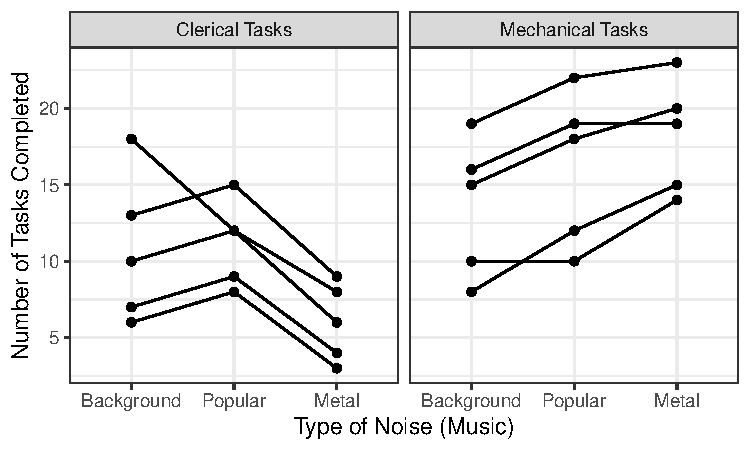
\includegraphics{Chapter-16-Assignment-R-Skeleton_files/figure-latex/unnamed-chunk-4-1} 

}

\caption{Person Profile Plot: Performance by Task Type and Noise}\label{fig:unnamed-chunk-4}
\end{figure}

\begin{figure}

{\centering 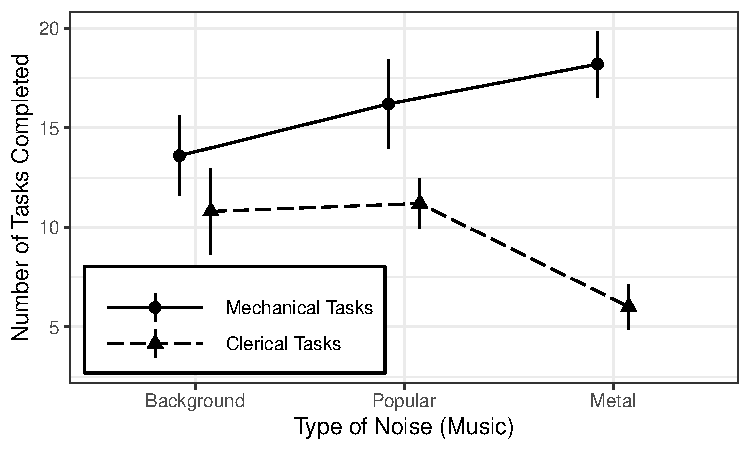
\includegraphics{Chapter-16-Assignment-R-Skeleton_files/figure-latex/unnamed-chunk-5-1} 

}

\caption{Group Means Plot: Performance by Task Type and Noise}\label{fig:unnamed-chunk-5}
\end{figure}

\clearpage

\hypertarget{question-b-4a-mixed-design-anova-display-all-sums-of-squares-components}{%
\subsubsection{Question B-4a Mixed Design ANOVA: display all
Sums-of-Squares
components}\label{question-b-4a-mixed-design-anova-display-all-sums-of-squares-components}}

\textbf{TEXTBOOK QUESTION:} \emph{(a) Perform a mixed-design ANOVA, and
display the results in a summary table.}

\textbf{DIRECTIONS:} Perform a Repeated Measures ANOVA for number of
tasks completed under the four noise conditions to see if there is an
effect and if the effect is different dependtion on the type of task.
Request no correction for violations of sphericity
(\texttt{correction\ =\ "none"}) and both effect sizes
(\texttt{es\ =\ c("ges",\ "pes"}). Make sure to save your model
(\texttt{fit\_tasks}), so that you can add \texttt{\$aov} at the end of
the name to extract all the Sums-of-Squares.

\begin{Shaded}
\begin{Highlighting}[]
\CommentTok{# Mixed ANOVA: display all Sums-of-Squares components}
\end{Highlighting}
\end{Shaded}

\clearpage

\hypertarget{question-b-4b-mixed-design-anova-effect-sizes}{%
\subsubsection{Question B-4b Mixed Design ANOVA: effect
sizes}\label{question-b-4b-mixed-design-anova-effect-sizes}}

\textbf{TEXTBOOK QUESTION:} \emph{(b) Calculate generalized eta squared
for the main effect of the type-of-task factor. Does this look like a
large effect size? Explain.}

\textbf{DIRECTIONS:} Run the name of the model \texttt{fit\_tasks} alone
to extract the adjusted degrees of freedom and F-test. The
sums-of-squares for the corrected test are the same as for the
uncorrected you just did.

\begin{Shaded}
\begin{Highlighting}[]
\CommentTok{# Mixed ANOVA: name the model was saved as}
\end{Highlighting}
\end{Shaded}

\begin{center}\rule{0.5\linewidth}{\linethickness}\end{center}

\textbf{Means Plot (model based)}

\textbf{DIRECTIONS:} Construct a means plot of \texttt{fit\_audience}
using \texttt{emmeans::emmip(\textasciitilde{}\ RM\_var)} to help
interpret the direction of any significant differences.

\begin{Shaded}
\begin{Highlighting}[]
\CommentTok{# RM ANOVA: means plot}
\end{Highlighting}
\end{Shaded}

\clearpage

\hypertarget{anograms_wide--repeated-measures-and-assigned-group-design-effect-of-music-and-task-type-on-production}{%
\subsection{\texorpdfstring{\texttt{anograms\_wide} -Repeated Measures
and Assigned Group Design: Effect of Music and Task Type on
Production}{anograms\_wide -Repeated Measures and Assigned Group Design: Effect of Music and Task Type on Production}}\label{anograms_wide--repeated-measures-and-assigned-group-design-effect-of-music-and-task-type-on-production}}

\textbf{TEXTBOOK QUESTION:} \emph{Dr.~Jones is investigating various
conditions that affect mental effort- which, in this experiment,
involves solving anagrams. Subjects were randomly assigned to one of
three experimental conditions. Subjects in the first group were told
that they would not be getting feedback on their performance. Subjects
in the second and third groups were told they would get feedback, but
only subjects in the third group were told (erroneously) that anagram
solving was highly correlated with intelligence and creativity
(Dr.~Jones hoped this information would produce ego involvement). The
list of anagrams given to each subject contained a random mix of
problems at four levels of difficulty determined by the number of
letters presented (five, six, seven, or eight). The number of anagrams
correctly solved by each subject in each condition and at each level of
difficulty is given in the following table:}

\hypertarget{restructure-from-wide-to-long-format-1}{%
\subsubsection{Restructure from wide to long
format:}\label{restructure-from-wide-to-long-format-1}}

\begin{verbatim}
         id         feedback difficulty correct
1    1_none      No Feedback   Length 5       9
2    1_none      No Feedback   Length 6       6
3    1_none      No Feedback   Length 7       4
4    1_none      No Feedback   Length 8       2
5      <NA>             <NA>       <NA>     ...
6 3_withEgo Feedback and Ego   Length 5      34
7 3_withEgo Feedback and Ego   Length 6      32
8 3_withEgo Feedback and Ego   Length 7      28
9 3_withEgo Feedback and Ego   Length 8      24
\end{verbatim}

\hypertarget{summary-statistics-1}{%
\subsubsection{Summary Statistics}\label{summary-statistics-1}}

\begin{table}[ ht ] 
\centering 
\caption{Descriptives: Performance by Feedback and Difficulty}\label{}
\begin{tabular}{ l c c c c }
\toprule
 &   &  \multicolumn{ 3 }{c}{ Randomized Condition }\\ 
  & Total & No Feedback & Only Feedback & Feedback and Ego \\ 
 & n = 9 & n = 3 & n = 3 & n = 3 \\ 
 \midrule
Length 5 &   &   &   &  \\ 
\hspace{6pt}   & 20.7 (9.4) & 10.3 (1.5) & 20.0 (1.7) & 31.7 (2.1)\\ 
Length 6 &   &   &   &  \\ 
\hspace{6pt}   & 17.8 (9.7) & 7.3 (1.5) & 17.0 (2.6) & 29.0 (3.6)\\ 
Length 7 &   &   &   &  \\ 
\hspace{6pt}   & 15.0 (9.3) & 5.0 (1.7) & 14.3 (3.1) & 25.7 (3.2)\\ 
Length 8 &   &   &   &  \\ 
\hspace{6pt}   & 12.8 (8.5) & 3.3 (1.5) & 12.3 (1.5) & 22.7 (1.5)\\ 
\bottomrule

\end{tabular}
\end{table}

\clearpage

\hypertarget{exploratory-visualizations}{%
\subsubsection{Exploratory
Visualizations}\label{exploratory-visualizations}}

\begin{figure}

{\centering 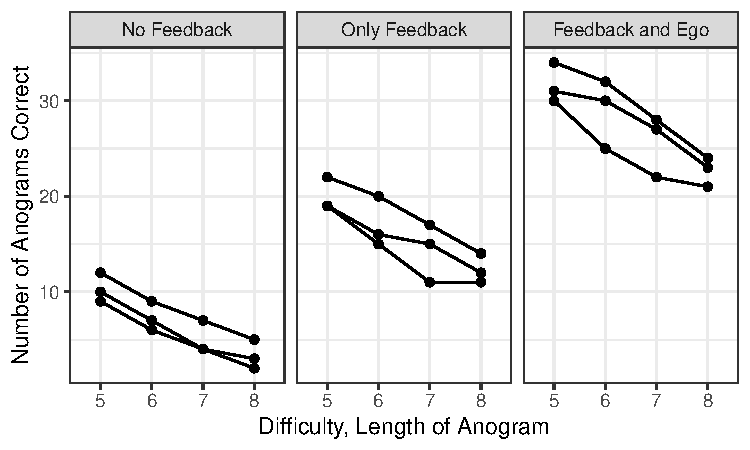
\includegraphics{Chapter-16-Assignment-R-Skeleton_files/figure-latex/unnamed-chunk-12-1} 

}

\caption{Person Profile Plot: Performance by Feedback and Difficulty}\label{fig:unnamed-chunk-12}
\end{figure}

\begin{figure}

{\centering 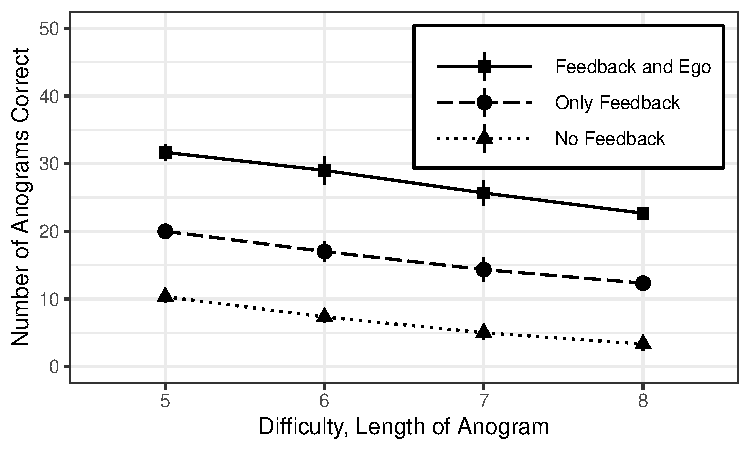
\includegraphics{Chapter-16-Assignment-R-Skeleton_files/figure-latex/unnamed-chunk-13-1} 

}

\caption{Group Means Plot: Performance by Feedback and Difficulty}\label{fig:unnamed-chunk-13}
\end{figure}

\clearpage

\hypertarget{question-b-5b-mixed-design-anova-display-all-sums-of-squares-components}{%
\subsubsection{Question B-5b Mixed Design ANOVA: display all
Sums-of-Squares
components}\label{question-b-5b-mixed-design-anova-display-all-sums-of-squares-components}}

\textbf{TEXTBOOK QUESTION:} \emph{(b) Perform a mixed analysis of
variance, and display the results in a summary table. Would any of your
conclusions change if you do not assume sphericity? Explain.}

\textbf{DIRECTIONS:} Perform a Repeated Measures ANOVA for number of
tasks completed under the four noise conditions to see if there is an
effect and if the effect is different dependtion on the type of task.
Make sure to save your model (\texttt{fit\_ano}), so that you can add
\texttt{\$aov} at the end of the name to extract all the
Sums-of-Squares.

\begin{Shaded}
\begin{Highlighting}[]
\CommentTok{# Mixed ANOVA: display all Sums-of-Squares components}
\end{Highlighting}
\end{Shaded}

\clearpage

\textbf{DIRECTIONS:} Use the \texttt{summary()} function on the model
name \texttt{fit\_ano} to display the sphericity test and corrections to
answer the last portion of this question.

\begin{Shaded}
\begin{Highlighting}[]
\CommentTok{# Mixed ANOVA: sphericity tests and corrections}
\end{Highlighting}
\end{Shaded}

\clearpage

\hypertarget{question-b-5c-mixed-design-anova-main-effects-post-hoc-with-appropriate-correction}{%
\subsubsection{Question B-5c Mixed Design ANOVA: Main Effect's post-hoc
with appropriate
correction}\label{question-b-5c-mixed-design-anova-main-effects-post-hoc-with-appropriate-correction}}

\textbf{TEXTBOOK QUESTION:} \emph{(c) Perform post hoc pairwise
comparisons for both main effects, using the appropriate error term from
part b in each case. Explain why these follow-up tests are appropriate
given your results in part b.}

\textbf{DIRECTIONS:} Use the prior model \texttt{fit\_ano} to run post
hoc test for the levels of each main effect, separately SINCE THE
INTERACTION IS NOT SIGNIFICANT (including a means plot). Choose an
appropriate method to control type I errors when making multiple
comparisons.

\begin{Shaded}
\begin{Highlighting}[]
\CommentTok{# Mixed ANOVA: post hoc pairwise tests <-- feedback}
\end{Highlighting}
\end{Shaded}

\begin{center}\rule{0.5\linewidth}{\linethickness}\end{center}

\begin{Shaded}
\begin{Highlighting}[]
\CommentTok{# RM ANOVA: means plot <--feedback}
\end{Highlighting}
\end{Shaded}

\clearpage

\begin{Shaded}
\begin{Highlighting}[]
\CommentTok{# Mixed ANOVA: post hoc pairwise tests <-- difficulty}
\end{Highlighting}
\end{Shaded}

\begin{center}\rule{0.5\linewidth}{\linethickness}\end{center}

\begin{Shaded}
\begin{Highlighting}[]
\CommentTok{# RM ANOVA: means plot <-- difficulty}
\end{Highlighting}
\end{Shaded}

\clearpage

\hypertarget{brain_wide---repeated-measures-and-observed-groups-design-differential-effect-of-stimuli-on-recall-by-brain-damage}{%
\subsection{\texorpdfstring{\texttt{brain\_wide} - Repeated Measures and
Observed Groups Design: Differential Effect of Stimuli on Recall, by
Brain
Damage}{brain\_wide - Repeated Measures and Observed Groups Design: Differential Effect of Stimuli on Recall, by Brain Damage}}\label{brain_wide---repeated-measures-and-observed-groups-design-differential-effect-of-stimuli-on-recall-by-brain-damage}}

\textbf{TEXTBOOK QUESTION:} \emph{Exercise 15B6 described a
neuropsychologist studying subjects with brain damage to the left
cerebral hemisphere. Such a study would probably include a group of
subjects with damage to the right hemisphere and a group of control
subjects without brain damage. The data from Exercise 15B6 (the number
of digit or letter strings each subject recalled) follow, along with
data for the two comparison groups just mentioned.}

\hypertarget{restructure-from-wide-to-long-format-2}{%
\subsubsection{Restructure from wide to long
format:}\label{restructure-from-wide-to-long-format-2}}

\begin{verbatim}
       id  damage stimuli longest_correct
1  1_left    Left  Digits               6
2  1_left    Left Letters               5
3  1_left    Left   Mixed               6
4 1_right   Right  Digits               9
5    <NA>    <NA>    <NA>             ...
6 6_right   Right   Mixed               9
7  6_none Neither  Digits              10
8  6_none Neither Letters              10
9  6_none Neither   Mixed               9
\end{verbatim}

\hypertarget{summary-statistics-2}{%
\subsubsection{Summary Statistics}\label{summary-statistics-2}}

\begin{table}[ ht ] 
\centering 
\caption{Descriptives: Recall by Hemisphere and Stimuli}\label{}
\begin{tabular}{ l c c c c }
\toprule
 &   &  \multicolumn{ 3 }{c}{ Hemisphere of Brain Damage }\\ 
  & Total & Left & Right & Neither \\ 
 & n = 18 & n = 6 & n = 6 & n = 6 \\ 
 \midrule
Digits &   &   &   &  \\ 
\hspace{6pt}   & 8.1 (1.2) & 7.0 (0.9) & 8.2 (1.0) & 9.0 (0.9)\\ 
Letters &   &   &   &  \\ 
\hspace{6pt}   & 7.3 (1.6) & 5.7 (1.2) & 7.5 (0.8) & 8.7 (1.2)\\ 
Mixed &   &   &   &  \\ 
\hspace{6pt}   & 7.2 (1.5) & 5.8 (1.5) & 7.5 (1.0) & 8.3 (0.8)\\ 
\bottomrule

\end{tabular}
\end{table}

\clearpage

\hypertarget{exploratory-visualizations-1}{%
\subsubsection{Exploratory
Visualizations}\label{exploratory-visualizations-1}}

\begin{figure}

{\centering 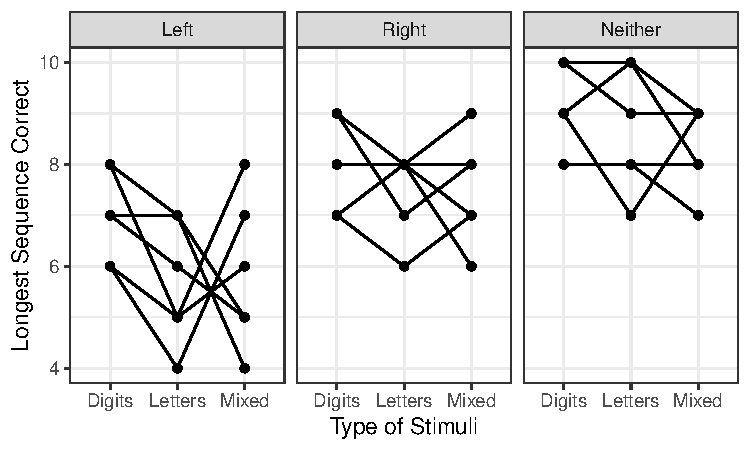
\includegraphics{Chapter-16-Assignment-R-Skeleton_files/figure-latex/unnamed-chunk-23-1} 

}

\caption{Person Profile Plot: Recall by Hemisphere and Stimul}\label{fig:unnamed-chunk-23}
\end{figure}

\begin{figure}

{\centering 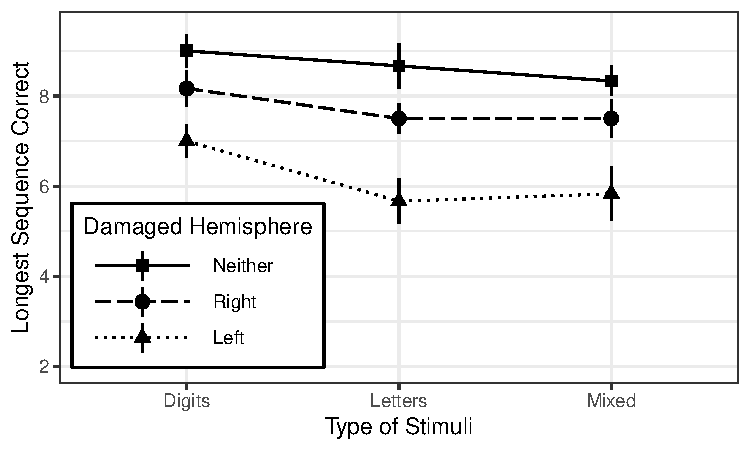
\includegraphics{Chapter-16-Assignment-R-Skeleton_files/figure-latex/unnamed-chunk-24-1} 

}

\caption{Group Means Plot: Recall by Hemisphere and Stimul}\label{fig:unnamed-chunk-24}
\end{figure}

\clearpage

\hypertarget{question-b-8a-b-mixed-design-anova-with-sphericity-test-and-corrections}{%
\subsubsection{Question B-8a-b Mixed Design ANOVA: with sphericity test
and
corrections}\label{question-b-8a-b-mixed-design-anova-with-sphericity-test-and-corrections}}

\textbf{TEXTBOOK QUESTION:} \emph{(a) Perform a mixed-design ANOVA and
test the three F ratios at the .05 level. What can you conclude about
the effects of brain damage on short-term recall for these types of
stimuli? (b) Draw a graph of these data, subject by subject. Do the
assumptions of the mixed-design ANOVA seem reasonable in this case?
Explain. }

\textbf{DIRECTIONS:} Perform a Repeated Measures ANOVA for longest
correct recall under the various stimuli to see if there is an effect
and if the effect is different dependtion on brain damage. Make sure to
save your model (\texttt{fit\_brain}), so that you can use the
\texttt{summary()} function on the name to test for sphericity and make
appropriate corrections.

\begin{Shaded}
\begin{Highlighting}[]
\CommentTok{# Mixed ANOVA:  with sphericity tests and corrections}
\end{Highlighting}
\end{Shaded}

\clearpage

\hypertarget{question-b-8c-mixed-design-anova-main-effects-post-hoc-with-appropriate-correction}{%
\subsubsection{Question B-8c Mixed Design ANOVA: Main Effect's post-hoc
with appropriate
correction}\label{question-b-8c-mixed-design-anova-main-effects-post-hoc-with-appropriate-correction}}

\textbf{TEXTBOOK QUESTION:} \emph{(c) Perform post hoc pairwise
comparisons for both main effects. Do not assume sphericity for the RM
factor.}

\textbf{DIRECTIONS:} Use the prior model \texttt{fit\_brain} to run post
hoc test for the levels of each main effect, separately SINCE THE
INTERACTION IS NOT SIGNIFICANT (including a means plot). Choose an
appropriate method to control type I errors when making multiple
comparisons. (you do not need to worry about sphericity)

\begin{Shaded}
\begin{Highlighting}[]
\CommentTok{# Mixed ANOVA: post hoc pairwise tests <-- damage}
\end{Highlighting}
\end{Shaded}

\begin{center}\rule{0.5\linewidth}{\linethickness}\end{center}

\begin{Shaded}
\begin{Highlighting}[]
\CommentTok{# RM ANOVA: means plot <-- damage}
\end{Highlighting}
\end{Shaded}

\clearpage

\begin{Shaded}
\begin{Highlighting}[]
\CommentTok{# Mixed ANOVA: post hoc pairwise tests <-- stimuli}
\end{Highlighting}
\end{Shaded}

\begin{center}\rule{0.5\linewidth}{\linethickness}\end{center}

\begin{Shaded}
\begin{Highlighting}[]
\CommentTok{# RM ANOVA: means plot <-- stimuli}
\end{Highlighting}
\end{Shaded}

\clearpage

\hypertarget{section-c}{%
\section{SECTION C}\label{section-c}}

\hypertarget{import-data-define-factors-and-compute-new-variables}{%
\subsection{Import Data, Define Factors, and Compute New
Variables}\label{import-data-define-factors-and-compute-new-variables}}

Import Data, Define Factors, and Compute New Variables

\begin{itemize}
\tightlist
\item
  Make sure the \textbf{dataset} is saved in the same \emph{folder} as
  this file
\item
  Make sure the that \emph{folder} is the \textbf{working directory}
\end{itemize}

\begin{quote}
NOTE: I added the second line to convert all the variables names to
lower case. I still kept the \texttt{F} as a capital letter at the end
of the five factor variables.
\end{quote}

\begin{Shaded}
\begin{Highlighting}[]
\NormalTok{ihno_clean <-}\StringTok{ }\KeywordTok{read_excel}\NormalTok{(}\StringTok{"Ihno_dataset.xls"}\NormalTok{) }\OperatorTok\StringTok{ }
\StringTok{  }\NormalTok{dplyr}\OperatorTok{::}\KeywordTok{rename_all}\NormalTok{(tolower) }\OperatorTok\StringTok{ }
\StringTok{  }\NormalTok{dplyr}\OperatorTok{::}\KeywordTok{mutate}\NormalTok{(}\DataTypeTok{genderF =}\NormalTok{ gender }\OperatorTok\StringTok{ }
\StringTok{                  }\KeywordTok{factor}\NormalTok{(}\DataTypeTok{levels =} \KeywordTok{c}\NormalTok{(}\DecValTok{1}\NormalTok{, }\DecValTok{2}\NormalTok{),}
                         \DataTypeTok{labels =} \KeywordTok{c}\NormalTok{(}\StringTok{"Female"}\NormalTok{, }
                                    \StringTok{"Male"}\NormalTok{))) }\OperatorTok\StringTok{ }
\StringTok{  }\NormalTok{dplyr}\OperatorTok{::}\KeywordTok{mutate}\NormalTok{(}\DataTypeTok{majorF =}\NormalTok{ major }\OperatorTok\StringTok{ }
\StringTok{                  }\KeywordTok{factor}\NormalTok{(}\DataTypeTok{levels =} \KeywordTok{c}\NormalTok{(}\DecValTok{1}\NormalTok{, }\DecValTok{2}\NormalTok{, }\DecValTok{3}\NormalTok{, }\DecValTok{4}\NormalTok{,}\DecValTok{5}\NormalTok{),}
                         \DataTypeTok{labels =} \KeywordTok{c}\NormalTok{(}\StringTok{"Psychology"}\NormalTok{,}
                                    \StringTok{"Premed"}\NormalTok{,}
                                    \StringTok{"Biology"}\NormalTok{,}
                                    \StringTok{"Sociology"}\NormalTok{,}
                                    \StringTok{"Economics"}\NormalTok{))) }\OperatorTok\StringTok{ }
\StringTok{  }\NormalTok{dplyr}\OperatorTok{::}\KeywordTok{mutate}\NormalTok{(}\DataTypeTok{reasonF =}\NormalTok{ reason }\OperatorTok\StringTok{ }
\StringTok{                  }\KeywordTok{factor}\NormalTok{(}\DataTypeTok{levels =} \KeywordTok{c}\NormalTok{(}\DecValTok{1}\NormalTok{, }\DecValTok{2}\NormalTok{, }\DecValTok{3}\NormalTok{),}
                         \DataTypeTok{labels =} \KeywordTok{c}\NormalTok{(}\StringTok{"Program requirement"}\NormalTok{,}
                                    \StringTok{"Personal interest"}\NormalTok{,}
                                    \StringTok{"Advisor recommendation"}\NormalTok{))) }\OperatorTok\StringTok{ }
\StringTok{  }\NormalTok{dplyr}\OperatorTok{::}\KeywordTok{mutate}\NormalTok{(}\DataTypeTok{exp_condF =}\NormalTok{ exp_cond }\OperatorTok\StringTok{ }
\StringTok{                  }\KeywordTok{factor}\NormalTok{(}\DataTypeTok{levels =} \KeywordTok{c}\NormalTok{(}\DecValTok{1}\NormalTok{, }\DecValTok{2}\NormalTok{, }\DecValTok{3}\NormalTok{, }\DecValTok{4}\NormalTok{),}
                         \DataTypeTok{labels =} \KeywordTok{c}\NormalTok{(}\StringTok{"Easy"}\NormalTok{,}
                                    \StringTok{"Moderate"}\NormalTok{,}
                                    \StringTok{"Difficult"}\NormalTok{,}
                                    \StringTok{"Impossible"}\NormalTok{))) }\OperatorTok\StringTok{ }
\StringTok{  }\NormalTok{dplyr}\OperatorTok{::}\KeywordTok{mutate}\NormalTok{(}\DataTypeTok{coffeeF =}\NormalTok{ coffee }\OperatorTok\StringTok{ }
\StringTok{                  }\KeywordTok{factor}\NormalTok{(}\DataTypeTok{levels =} \KeywordTok{c}\NormalTok{(}\DecValTok{0}\NormalTok{, }\DecValTok{1}\NormalTok{),}
                         \DataTypeTok{labels =} \KeywordTok{c}\NormalTok{(}\StringTok{"Not a regular coffee drinker"}\NormalTok{,}
                                    \StringTok{"Regularly drinks coffee"}\NormalTok{)))}
\end{Highlighting}
\end{Shaded}

\clearpage

\hypertarget{ihno_clean---repeated-measures-and-observed-group-design-differential-effect-of-a-pop-quiz-time-baseline-pre-quiz-post-quiz-on-anxiety-anxiety-by-major-majorf}{%
\subsection{\texorpdfstring{\texttt{ihno\_clean} - Repeated Measures and
Observed Group Design: Differential Effect of a Pop Quiz (time =
Baseline, pre-quiz, post-quiz) on Anxiety (anxiety), by Major
(majorF)}{ihno\_clean - Repeated Measures and Observed Group Design: Differential Effect of a Pop Quiz (time = Baseline, pre-quiz, post-quiz) on Anxiety (anxiety), by Major (majorF)}}\label{ihno_clean---repeated-measures-and-observed-group-design-differential-effect-of-a-pop-quiz-time-baseline-pre-quiz-post-quiz-on-anxiety-anxiety-by-major-majorf}}

\hypertarget{question-c-1a-mixed-design-anova-with-main-effect-post-hocs}{%
\subsubsection{Question C-1a Mixed Design ANOVA: with main effect post
hocs}\label{question-c-1a-mixed-design-anova-with-main-effect-post-hocs}}

\textbf{TEXTBOOK QUESTION:} \emph{(a) Perform a mixed-design ANOVA with
the three anxiety measures as the RM levels, and major as the
between-subjects factor. Request a plot of the cell means, \sout{and
post hoc tests for both the RM factor (LSD) and for major (Tukey)}.
Report the results of the ANOVA in APA style.}

Restructure from wide to long format:

\begin{Shaded}
\begin{Highlighting}[]
\NormalTok{ihno_anx_long <-}\StringTok{ }\NormalTok{ihno_clean }\OperatorTok\StringTok{ }
\StringTok{  }\NormalTok{tidyr}\OperatorTok{::}\KeywordTok{pivot_longer}\NormalTok{(}\DataTypeTok{cols =} \KeywordTok{c}\NormalTok{(anx_base, anx_pre, anx_post),}
                      \DataTypeTok{names_to =} \StringTok{"time"}\NormalTok{,}
                      \DataTypeTok{names_prefix =} \StringTok{"anx_"}\NormalTok{,}
                      \DataTypeTok{names_ptypes =} \KeywordTok{list}\NormalTok{(}\DataTypeTok{time =} \KeywordTok{factor}\NormalTok{()),}
                      \DataTypeTok{values_to =} \StringTok{"anxiety"}\NormalTok{)}
\end{Highlighting}
\end{Shaded}

\begin{Shaded}
\begin{Highlighting}[]
\NormalTok{ihno_anx_long }\OperatorTok\StringTok{ }
\StringTok{  }\NormalTok{dplyr}\OperatorTok{::}\KeywordTok{select}\NormalTok{(sub_num, majorF, time, anxiety) }\OperatorTok\StringTok{ }
\StringTok{  }\NormalTok{psych}\OperatorTok{::}\KeywordTok{headTail}\NormalTok{()}
\end{Highlighting}
\end{Shaded}

\begin{verbatim}
  sub_num     majorF time anxiety
1       1 Psychology base      17
2       1 Psychology  pre      22
3       1 Psychology post      20
4       2 Psychology base      17
5     ...       <NA> <NA>     ...
6      99  Economics post      18
7     100  Economics base      17
8     100  Economics  pre      11
9     100  Economics post      14
\end{verbatim}

\textbf{DIRECTIONS:} Using the \texttt{ihno\_anx\_long} dataset
restructured above, perform a Repeated Measures ANOVA for at the three
time points to see if the experiment had an effect on anxiety and if the
effect is different dependtion on major. Make sure to save your model
(\texttt{fit\_anx\_major}), so that you can use the \texttt{summary()}
function on the name to test for sphericity and make appropriate
corrections. Do specify that you would like to display BOTH effect size
measures with \texttt{es\ =\ c("ges",\ "pes")}, but do NOT include
\texttt{correction\ =\ "none"}.

\begin{Shaded}
\begin{Highlighting}[]
\CommentTok{# Mixed ANOVA:  with sphericity tests and corrections}
\end{Highlighting}
\end{Shaded}

\clearpage

\textbf{DIRECTIONS:} To display the effect size meausre, run the name
(\texttt{fit\_anx\_major}) of the model alone.

\begin{Shaded}
\begin{Highlighting}[]
\CommentTok{# Mixed ANOVA: effect sizes }
\end{Highlighting}
\end{Shaded}

\begin{center}\rule{0.5\linewidth}{\linethickness}\end{center}

\textbf{DIRECTIONS:} SINCE THE INTERACTIONIS SIGNIFICANT, instead of
focusing on the main effects alone, plot the interaction with the
\texttt{emmeans::emmip(group\_var\ \textasciitilde{}\ RM\_var)}
function.

\begin{Shaded}
\begin{Highlighting}[]
\CommentTok{# Mixed ANOVA: means plot <-- interaction}
\end{Highlighting}
\end{Shaded}

\clearpage

\hypertarget{ihno_clean---repeated-measures-and-observed-group-design-differential-effect-of-a-pop-quiz-time-baseline-pre-quiz-post-quiz-on-heart-rate-heart_rate-by-gender-genderf}{%
\subsection{\texorpdfstring{\texttt{ihno\_clean} - Repeated Measures and
Observed Group Design: Differential Effect of a Pop Quiz (time =
Baseline, pre-quiz, post-quiz) on Heart Rate (heart\_rate), by Gender
(genderF)}{ihno\_clean - Repeated Measures and Observed Group Design: Differential Effect of a Pop Quiz (time = Baseline, pre-quiz, post-quiz) on Heart Rate (heart\_rate), by Gender (genderF)}}\label{ihno_clean---repeated-measures-and-observed-group-design-differential-effect-of-a-pop-quiz-time-baseline-pre-quiz-post-quiz-on-heart-rate-heart_rate-by-gender-genderf}}

\hypertarget{question-c-2a-mixed-design-anova-with-main-effect-post-hocs}{%
\subsubsection{Question C-2a Mixed Design ANOVA: with main effect post
hocs}\label{question-c-2a-mixed-design-anova-with-main-effect-post-hocs}}

\textbf{TEXTBOOK QUESTION:} \emph{(a) Perform a mixed-design ANOVA with
the three heart-rate measures as the RM levels and gender as the
between-subjects factor. Request a plot of the cell means and post hoc
tests for the RM factor (LSD). Report the results of the ANOVA in APA
style.}

Restructure from wide to long format:

\begin{Shaded}
\begin{Highlighting}[]
\NormalTok{ihno_hr_long <-}\StringTok{ }\NormalTok{ihno_clean }\OperatorTok\StringTok{ }
\StringTok{  }\NormalTok{tidyr}\OperatorTok{::}\KeywordTok{pivot_longer}\NormalTok{(}\DataTypeTok{cols =} \KeywordTok{c}\NormalTok{(hr_base, hr_pre, hr_post),}
                      \DataTypeTok{names_to =} \StringTok{"time"}\NormalTok{,}
                      \DataTypeTok{names_prefix =} \StringTok{"hr_"}\NormalTok{,}
                      \DataTypeTok{names_ptypes =} \KeywordTok{list}\NormalTok{(}\DataTypeTok{time =} \KeywordTok{factor}\NormalTok{()),}
                      \DataTypeTok{values_to =} \StringTok{"heart_rate"}\NormalTok{)}
\end{Highlighting}
\end{Shaded}

\begin{Shaded}
\begin{Highlighting}[]
\NormalTok{ihno_hr_long }\OperatorTok\StringTok{ }
\StringTok{  }\NormalTok{dplyr}\OperatorTok{::}\KeywordTok{select}\NormalTok{(sub_num, genderF, time, heart_rate) }\OperatorTok\StringTok{ }
\StringTok{  }\NormalTok{psych}\OperatorTok{::}\KeywordTok{headTail}\NormalTok{()}
\end{Highlighting}
\end{Shaded}

\begin{verbatim}
  sub_num genderF time heart_rate
1       1  Female base         71
2       1  Female  pre         68
3       1  Female post         65
4       2  Female base         73
5     ...    <NA> <NA>        ...
6      99    Male post         73
7     100    Male base         70
8     100    Male  pre         70
9     100    Male post         64
\end{verbatim}

\clearpage

\textbf{DIRECTIONS:} Using the \texttt{ihno\_hr\_long} dataset just
reformatted, perform a Repeated Measures ANOVA for at the three time
points to see if the experiment had an effect on heart rateand if the
effect is different dependtion on gender Make sure to save your model
(\texttt{fit\_hr\_gender}), so that you can use the \texttt{summary()}
function on the name to test for sphericity and make appropriate
corrections. Do specify that you would like to display BOTH effect size
measures with \texttt{es\ =\ c("ges",\ "pes")}, but do NOT include
\texttt{correction\ =\ "none"}.

\begin{Shaded}
\begin{Highlighting}[]
\CommentTok{# Mixe ANOVA:  with sphericity tests and corrections}
\end{Highlighting}
\end{Shaded}

\clearpage

\textbf{DIRECTIONS:} Use the prior model \texttt{fit\_hr\_gender} to run
post hoc test for the levels of each main effect, separately SINCE THE
INTERACTION IS \textbf{NOT} SIGNIFICANT (including a means plot). Choose
an appropriate method to control type I errors when making multiple
comparisons. You do not need to worry about sphericity since there are
only 2 time points. Also, you do not need to worry about follow-up tests
for gender, since it only has 2 levels.

\begin{Shaded}
\begin{Highlighting}[]
\CommentTok{# Mixed ANOVA: post hoc pairwise tests <-- time}
\end{Highlighting}
\end{Shaded}

\begin{center}\rule{0.5\linewidth}{\linethickness}\end{center}

\begin{Shaded}
\begin{Highlighting}[]
\CommentTok{# RM ANOVA: means plot <-- time}
\end{Highlighting}
\end{Shaded}

\clearpage

\hypertarget{ihno_clean---repeated-measures-and-assigned-group-design-differential-effect-of-the-experiemnt-quiz_type-pop-quiz-vs.-standard-quiz-on-quiz-score-quiz_score-by-difficulty-level-exp_condf}{%
\subsection{\texorpdfstring{\texttt{ihno\_clean} - Repeated Measures and
Assigned Group Design: Differential Effect of the Experiemnt (quiz\_type
= Pop Quiz vs.~Standard Quiz) on Quiz Score (quiz\_score), by Difficulty
Level
(exp\_condF)}{ihno\_clean - Repeated Measures and Assigned Group Design: Differential Effect of the Experiemnt (quiz\_type = Pop Quiz vs.~Standard Quiz) on Quiz Score (quiz\_score), by Difficulty Level (exp\_condF)}}\label{ihno_clean---repeated-measures-and-assigned-group-design-differential-effect-of-the-experiemnt-quiz_type-pop-quiz-vs.-standard-quiz-on-quiz-score-quiz_score-by-difficulty-level-exp_condf}}

\hypertarget{question-c-3a-mixed-design-anova-is-there-an-interaction}{%
\subsubsection{Question C-3a Mixed Design ANOVA: is there an
interaction?}\label{question-c-3a-mixed-design-anova-is-there-an-interaction}}

\textbf{TEXTBOOK QUESTION:} \emph{(a) Perform a mixed-design ANOVA with
the two 10-point quizzes (statquiz and exp\_sqz) as the RM levels, and
exp\_cond as the between-subjects factor. Request a plot of the cell
means. Report the results of the ANOVA in APA style. If the interaction
is significant, explain the pattern you see in the plot of the cell
means.}

Restructure from wide to long format:

\begin{Shaded}
\begin{Highlighting}[]
\NormalTok{ihno_statquiz_long <-}\StringTok{ }\NormalTok{ihno_clean }\OperatorTok\StringTok{ }
\StringTok{  }\NormalTok{tidyr}\OperatorTok{::}\KeywordTok{pivot_longer}\NormalTok{(}\DataTypeTok{cols =} \KeywordTok{c}\NormalTok{(statquiz, exp_sqz),}
                      \DataTypeTok{names_to =} \StringTok{"quiz_type"}\NormalTok{,}
                      \DataTypeTok{names_ptypes =} \KeywordTok{list}\NormalTok{(}\DataTypeTok{time =} \KeywordTok{factor}\NormalTok{()),}
                      \DataTypeTok{values_to =} \StringTok{"quiz_score"}\NormalTok{) }\OperatorTok\StringTok{ }
\StringTok{  }\NormalTok{dplyr}\OperatorTok{::}\KeywordTok{mutate}\NormalTok{(}\DataTypeTok{quiz_type =}\NormalTok{ quiz_type }\OperatorTok\StringTok{ }
\StringTok{                  }\NormalTok{forcats}\OperatorTok{::}\KeywordTok{fct_recode}\NormalTok{(}\StringTok{"Regular"}\NormalTok{ =}\StringTok{ "statquiz"}\NormalTok{,}
                                      \StringTok{"Experimental"}\NormalTok{ =}\StringTok{ "exp_sqz"}\NormalTok{))}
\end{Highlighting}
\end{Shaded}

\begin{Shaded}
\begin{Highlighting}[]
\NormalTok{ihno_statquiz_long }\OperatorTok\StringTok{ }
\StringTok{  }\NormalTok{dplyr}\OperatorTok{::}\KeywordTok{select}\NormalTok{(sub_num, exp_condF, quiz_type, quiz_score) }\OperatorTok\StringTok{ }
\StringTok{  }\NormalTok{psych}\OperatorTok{::}\KeywordTok{headTail}\NormalTok{()}
\end{Highlighting}
\end{Shaded}

\begin{verbatim}
  sub_num  exp_condF    quiz_type quiz_score
1       1       Easy      Regular          6
2       1       Easy Experimental          7
3       2       Easy      Regular          9
4       2       Easy Experimental         11
5     ...       <NA>         <NA>        ...
6      99 Impossible      Regular          8
7      99 Impossible Experimental          8
8     100   Moderate      Regular          7
9     100   Moderate Experimental          7
\end{verbatim}

\textbf{DIRECTIONS:} Using the \texttt{ihno\_statquiz\_long} dataset
restructured above, perform a Repeated Measures ANOVA for at the two
quizes to see if the experiment had an effect on score and if the effect
is different dependtion on difficulty level. Make sure to save your
model (\texttt{fit\_quiz\_cond}), so that you can use the
\texttt{summary()} function on the name to view the output. Do specify
that you would like to display BOTH effect size measures with
\texttt{es\ =\ c("ges",\ "pes")}, but do NOT include
\texttt{correction\ =\ "none"}.

\begin{quote}
NOTE: When the measure is only repeated twice, sphericity can not be
violated, so no such test are performed.
\end{quote}

\begin{Shaded}
\begin{Highlighting}[]
\CommentTok{# Mixed ANOVA:  with summary}
\end{Highlighting}
\end{Shaded}

\clearpage

\textbf{DIRECTIONS:} SINCE THE INTERACTIONIS SIGNIFICANT, instead of
focusing on the main effects alone, plot the interaction with the
\texttt{emmeans::emmip(group\_var\ \textasciitilde{}\ RM\_var)}
function.

\begin{Shaded}
\begin{Highlighting}[]
\CommentTok{# RM ANOVA: means plot <-- interaction}
\end{Highlighting}
\end{Shaded}

\end{document}
